\subsection{Descripción}
Se tienen n servidores interconectados mediante m enlaces. Los enlaces tienen un costo en función del tráfico que transmiten y todos los enlaces deben transmitir la misma información. El problema a resolver consiste en seleccionar aquellos enlaces que permitan distribuir la información a los n nodos con costo total mínimo.


Veamos un ejemplo; el siguiente grafo tiene como solución el subgrafo en rojo con peso total 38.

\begin{center}
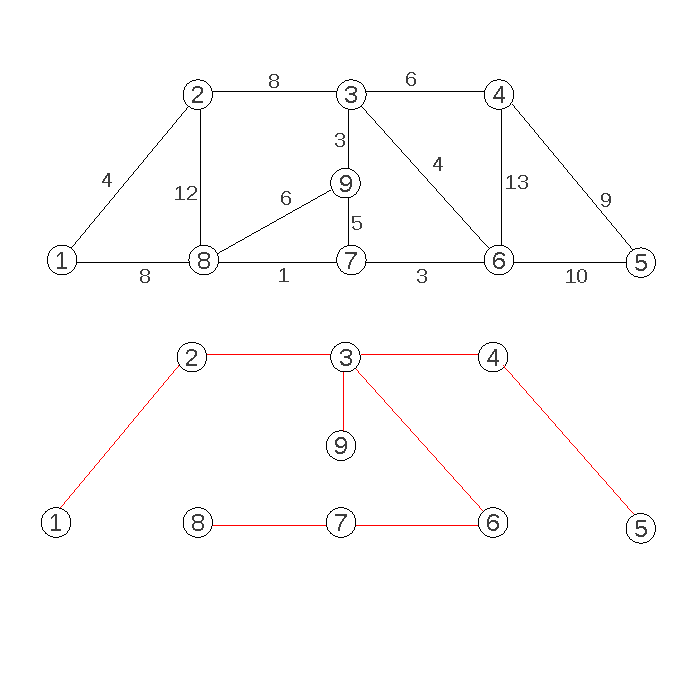
\includegraphics{ej2/1/Img1.pdf} 
\end{center}

